\subsubsection{Anwendungsszenario}
Dieser Abschnitt beschreibt die Anforderungen an das Softwaresystem mittels Anwendungsfällen und 
beschreibt die technischen Rahmenbedingungen, in dem das Softwaresystem eingebettet ist.
\subsubsection{Use Cases}

Die Anwendungsfälle beschreiben die Arbeit mit dem \textit{One-Million-Song}-Datensatz. 

Das Anwendungsfalldiagramm \ref{anforderungen:usecasediagramm} zeigt alle Anwendungsfälle für
die Arbeit mit dem Million-Song-Datensatz auf dem Hochschul-Cluster.

\begin{figure}[H]
	\centering
	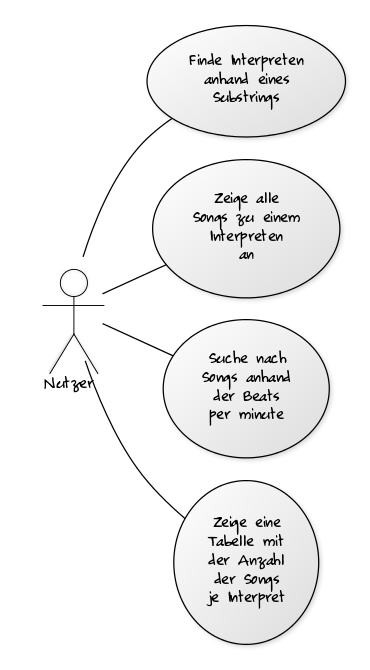
\includegraphics[width=0.5\textwidth]{images/06usecases.png}
	\caption{Anwendungsfall-Diagramm, UML 2.0. Alle Anwendungsfälle für das Million-Song-Projekt}
	\label{anforderungen:usecasediagramm}
\end{figure}

Es folgt eine kurze Beschreibung der einzelnen Anwendungsfälle. Auf eine detaillierte Ausarbeitung im Rahmen einer 
ausführlichen Anforderungsanalyse soll in diesem Falle verzichtet werden, weil ein konkretes Anwendungsszenario fehlt und
die Anwendungsfälle künstlicher Natur sind, um den Einsatz von Hadoop, MapReduce und Hbase im Bereich einer
Big-Data-Anwendung zu evaluieren.

\begin{description}
	\item[UC 1] Der Nutzer möchte eine Motto-Party veranstalten. Er kann sich allerdings nicht mehr genau an den Namen des Interpreten erinnern. Mit Hilfe der Vorschläge, die ihm dynamisch während des Tippens angezeigt werden, ist es ihm möglich den Interpreten zu finden.
	\item[UC 2] Der Nutzer möchte nun alle Songs zu einem Interpreten aus \textbf{UC 1} anzeigen.
	\item[UC 3] Der Nutzer möchte ein speziell für ihn angepasstes Lauftraining absolvieren. Dazu sucht er nach Songs mit einer speziellen \ac{BPM}-Rate.
	\item[UC 4] Der Nutzer möchte nach besonders erfolgreichen Interpreten in der Datenbank suchen. Daher lässt er sich eine Tabelle ausgeben, in der die Songs pro Interpret dargestellt werden.

\end{description}

\subsubsection{Parametriesierbarkeit}
\label{anforderungen:rahmenbedingungen}
Die Rahmenbedingungen teilen sich in die Hardware-Rahmenbedingungen und in die Software-Rahmenbedingungen auf.
Die Hardware, die uns zur Verfügung gestellt wurde besteht aus einem Verbund von 5 homogenen Server-Rechnern, 
die über ein Ethernet-Netzwerk gleichwertig miteinander verknüpft sind. Physikalisch sind alle Knoten an einem gemeinsamen
Switch angeschlossen als physikalische Stern-Topologie. Dies hat aus logischer Sicht zur Folge, dass eine direkte Kommunikation
zwischen den Knoten möglich ist. Die Bandbreite des gesamten Netzwerkes ist mit 20Mbit/s angegeben, was durch die Topologie
auch zwischen den einzelnen Knoten möglich wäre.

Die Server-Knoten sind alle mit folgender Hardware ausgestattet:
\begin{itemize}
	\item Intel i7-4790K CPU
	\item 32 GB RAM
	\item 256 GB SSD
	\item 2 TB HDD
\end{itemize}

Auf der Seite der Software ist auf allen Knoten mit \textit{Ubuntu} eine Linux-Distribution in der Version 
\textit{16.04.1 LTS Server 64-Bit} installiert. Root-Rechte sind gewährt.
Anzumerken ist, dass alle Ressourcen mit 9 anderen Teams geteilt werden und alle Teams auf der selben 
Instanz des Betriebssystems arbeiten und nur durch unterschiedliche Nutzer getrennt sind. 
Diese Rahmenbedingung ist insbesondere bei der Konfiguration der Netzwerk-Ports bei verteilten Anwendungen 
zu beachten, da verschiedene Anwendungen eventuell auf dem gleichen Port lauschen und somit 
Konflikte entstehen können.

\subsubsection{Installation und Konfiguration}
Auf dem Cluster wird das komplette Hadoop-Softwarepaket installiert, bestehend aus den
Komponenten \ac{YARN}, \ac{HDFS} und MapReduce. Installiert wird über einen Tarball von der offiziellen
Apache-Webseite (\url{http://www-us.apache.org/dist/hadoop/common/hadoop-2.7.3/hadoop-2.7.3.tar.gz}), um die aktuellste Version ($2.7.3$) von Hadoop zu erhalten. Die Installation selbst gestaltet sich mit dem Entpacken der Binär-Dateien im home-Verzeichnis 
denkbar einfach. Komplexer gestaltet sich die Konfiguration, die das Laufzeitverhalten der Komponenten festlegen.

Die folgenden Tabellen zeigen die Konfiguration der einzelnen Hadoop-Komponenten, die vom Standard abweicht.
Eine Auflistung der ab Werk ausgelieferten Standard-Konfiguration kann auf folgenden Webseiten nachgeschlagen werden:
\cite{hdfsDefault}, \cite{yarnDefault}, \cite{mapreduceDefault} \cite{hbaseConfig}.

Es folgen nun die Tabellen, die die Konfiguration von Hadoop, HDFS, YARN, MapReduce und HBase 
speziell für die vorhandene Cluster-Umgebung zeigen. Es werden  nur Parameter aufgelistet, 
die von der Werks-Konfiguration abweichen.

Hbase liefert von Haus aus bereits eine eigene ZooKeeper-Installation mit. Der Grund für eine eigene, getrennte ZooKeeper-Installation lag in der sauberen Trennung zwischen der Hbase-Konfiguration und der ZooKeeper-Konfiguration. 

\begin{table}
	\begin{tabularx}{\textwidth}{| X | X |} \hline
		Name des Parameters & Gesetzter Wert \\ \hline
		dfs.namenode.name.dir & file:/data/team6/namenode \\ \hline
		dfs.namenode.http-address & 10.20.110.61:50071  \\ \hline
		dfs.datanode.data.dir & file:/data/team6/datanode \\ \hline
		dfs.datanode.address & hdfs://localhost:5001 \\ \hline
		dfs.datanode.http-address & localhost:50016 \\ \hline
		dfs.datanode.ipc.address & localhost:50026 \\ \hline
	\end{tabularx}
	\caption{Gesetzte Parameter-Werte für die Konfiguration des HDFS}
	\label{config:hdfsValues}
\end{table}

\begin{table}
	\begin{tabularx}{\textwidth}{|X|X|} \hline
		Name des Parameters & Beschreibung \\ \hline
		dfs.namenode.name.dir & Lokaler Dateisystempfad, wo
		HDFS den Log für die Transaktionen ablegen soll. \\ \hline
		dfs.namenode.http-address & Die Web-Adresse, über den die
		Weboberfläche des HDFS-Überwachungswerkzeug erreichbar ist. \\ \hline
		dfs.datanode.data.dir & Lokaler Dateisystempfad, wo HDFS
		die Daten des virtuelle Dateisystems ablegen soll. \\ \hline
		dfs.datanode.address & Die Netzwerk-Schnittstelle, über den 
		der Datanode des Rechnerknotens über das hdfs-Protokoll erreichbar ist. Darüber 
		werden die Daten zwischen den Knoten des HDFS-Dateisystems ausgetauscht. \\ \hline
		dfs.datanode.http-address & Die Web-Adresse der Datanode-
		Adminoberfläche. \\ \hline
		dfs.datanode.ipc.address & Der Zugang zum Datanode mittels dem
		leichtgewichtigem IPC-Protokoll, über den Meta-Informationen des Dateisystems 
		ausgetauscht werden. \\ \hline
	\end{tabularx}
	\caption{Beschreibung der Konfigurations-Parameter des HDFS}
	\label{config:hdfsDescription}
\end{table}

\begin{table}
	\begin{tabularx}{\textwidth}{| X | X |} \hline
	yarn.resourcemanager.hostname & 10.20.110.61 \\ \hline
	yarn.resourcemanager.address & \$\{yarn.resourcemanager.hostname\}:8036 \\ \hline
	yarn.resourcemanager.scheduler & \$\{yarn.resourcemanager.hostname\}:8032 \\ \hline
	yarn.resourcemanager.webapp.address & \$\{yarn.resourcemanager.hostname\}:8086 \\ \hline
	yarn.resourcemanager.admin.address & \$\{yarn.resourcemanager.hostname\}:8037 \\ \hline
	yarn.nodemanager.address & \$\{yarn.nodemanager.hostname\}:8056 \\ \hline
	yarn.nodemanager.localizer.address & \$\{yarn.nodemanager.hostname\}:8046 \\ \hline
	yarn.nodemanager.resource.memory-mb & 4608 \\ \hline
	yarn.scheduler.minimum-allocation-mb & 1536 \\ \hline
	yarn.scheduler.maximum-allocation-mb & 4608 \\ \hline
	yarn.nodemanager.resource.percentage-physical-cpu-limit & 50 \\ \hline
	\end{tabularx}
	\caption{Gesetzte Parameter-Werte für die Konfiguration von YARN}
	\label{config:yarnValues}
\end{table}

\begin{table}
	\begin{tabularx}{\textwidth}{| X | X |} \hline
	yarn.resourcemanager.hostname & Der Standort des Resourcemanager von YARN \\ \hline
	yarn.resourcemanager.address &  Der Netzwerk-Port des Resourcemanagers, über den YARN-Jobs gestartet werden können.\\ \hline
	yarn.resourcemanager.scheduler & Die Netzwerk-Schnittstelle des Schedulers\\ \hline
	yarn.resourcemanager.webapp.address & Die Adresse der YARN-Weboberfläche\\ \hline
	yarn.resourcemanager.admin.address & Die Netzwerk-Schnittstelle zum Administrieren des YARN-Resourcemanagers\\ \hline
	yarn.nodemanager.address & Die Netzwerk-Schnittstelle des Nodemanagers von YARN auf den Rechnerknoten\\ \hline
	yarn.nodemanager.localizer.address & Die Netzwerk-Schnittstelle, über die mittels IPC
	Informationen über verfügbare Resourcen von den Rechnerknoten gesammelt wird.\\ \hline
	yarn.nodemanager.resource.memory-mb &  Menge an Speicher, die für einen Container reserviert werden kann.\\ \hline
	yarn.scheduler.minimum-allocation-mb &  Die minimale Menge an Speicher, die vom Resourcemanager für Container angefragt wird\\ \hline
	yarn.scheduler.maximum-allocation-mb &  Die maximale Menge an Speicher, die vom Resourcemanager für Container angefragt wird\\ \hline
	yarn.nodemanager.resource.percentage-physical-cpu-limit & Die maximale Beanspruchung der Rechenkapazität in Prozent insgesamt für alle Container auf einem Knoten. \\ \hline
	\end{tabularx}
	\caption{Beschreibung der Konfigurations-Parameter von YARN}
	\label{config:yarnDescription}
\end{table}

\begin{table}
	\begin{tabularx}{\textwidth}{| X | X |} \hline
	mapreduce.jobhistory.address & 0.0.0.0:10026 \\ \hline
	mapreduce.jobhistory.webapp.address & 0.0.0.0:19886 \\ \hline
	mapreduce.jobhistory.admin.address & 0.0.0.0:10036 \\ \hline
	mapreduce.cluster.local.dir & /data/team6/intermediate \\ \hline
	mapreduce.framework.name & yarn \\ \hline
	mapreduce.map.memory.mb & 1536 \\ \hline
	mapreduce.map.java.opts & -Xmx1228m \\ \hline
	mapreduce.reduce.memory.mb & 3072 \\ \hline
	mapreduce.reduce.java.opts & -Xmx2457m \\ \hline
	yarn.app.mapreduce.am.resource.mb & 3072 \\ \hline
	yarn.app.mapreduce.am.command-opts & -Xmx2457m \\ \hline
	\end{tabularx}
	\caption{Gesetzte Parameter-Werte für die Konfiguration von MapReduce}
	\label{config:mapreduceValues}
\end{table}

\begin{table}
	\begin{tabularx}{\textwidth}{| X | X |} \hline
	mapreduce.jobhistory.address & Die Netzwerk-Schnittstelle mittels dessen Informationen
	über laufende Jobs auf dem Rechnerknoten abgerufen werden können. \\ \hline
	mapreduce.jobhistory.webapp.address & Die Web-Oberfläche für die Betrachtung
	der laufenden MapReduce-Jobs auf dem Rechnerknoten.\\ \hline
	mapreduce.jobhistory.admin.address & Die Netzwerk-Schnittstelle für den Admin für
	Informationen über MapReduce-Jobs.\\ \hline
	mapreduce.cluster.local.dir &  Lokaler Dateipfad, wo die Zwischen-Ergebnisse des MapReduce-Jobs gespeichert werden sollen.\\ \hline
	mapreduce.framework.name &  Spezifiziert, welches konkretes MapReduce-Framework
	verwendet werden soll. \\ \hline
	mapreduce.map.memory.mb &  Verfügbarer Speicher für Map-Jobs\\ \hline
	mapreduce.map.java.opts & Spezifische Java-Optionen. Hier in diesem Falle die Erweiterung
	des verfügbaren Heap-Speichers für die Java-Prozesse von Map-Jobs.\\ \hline
	mapreduce.reduce.memory.mb &  Verfügbarer Speicher für Reduce-Jobs.\\ \hline
	mapreduce.reduce.java.opts & Spezifische Java-Optionen. Hier in diesem Falle die Erweiterung
	des verfügbaren Heap-Speichers für die Java-Prozesse von Reduce-Jobs. \\ \hline
	yarn.app.mapreduce.am.resource.mb & Die Menge an Speicher, die der AppMaster von
	Map-Reduce verwenden kann. \\ \hline
	yarn.app.mapreduce.am.command-opts &  Spezifische Java-Optionen für den AppMaster
	von Map-Reduce, in dem Falle die Erweiterung des Heap-Speichers.\\ \hline
	\end{tabularx}
	\caption{Beschreibung der Konfigurations-Parameter von MapReduce}
	\label{config:mapreduceDescription}
\end{table}

\begin{table}
	\begin{tabularx}{\textwidth}{| X | X |} \hline
	hbase.rootdir & hdfs://10.20.110.61:8026/hbase \\ \hline
	hbase.master.hostname & 10.20.110.61 \\ \hline
	hbase.master.port & 16006 \\ \hline
	hbase.cluster.distributed & true \\ \hline
	hbase.zookeeper.property.clientPort & 2186 \\ \hline
	hbase.zookeeper.quorum & $10.20.110.61$, $10.20.110.43$, $10.20.110.41$, $10.20.110.39$, $10.20.110.48$ \\ \hline
	\end{tabularx}
	\caption{Gesetzte Parameter-Werte für die Konfiguration von Hbase}
	\label{config:hbaseValues}
\end{table}

\begin{table}
	\begin{tabularx}{\textwidth}{| X | X |} \hline
	hbase.rootdir &  Hbase benötigt die Adresse eines Filesystems, wo es die Tabellen ablegen kann. In dem Projekt ist es das installierte
	HDFS-Dateisystem, dessen Zugang über den Namenode des Masters erfolgt.\\ \hline
	hbase.master.hostname & Angabe, auf welchem Rechner-Knoten der Masternode liegen soll.\\ \hline
	hbase.master.port & Der Port, auf dem der Masternode für die Datanodes von Hbase ansprechbar ist. \\ \hline
	hbase.cluster.distributed & Hbase kann entweder als Stand-Alone-Anwendung auf einem Knoten laufen (\textit{false}) oder als verteilte
	 Anwendung (\textit{true}). \\ \hline
	hbase.zookeeper.property.clientPort & Hbase benötigt im verteilten Modus zwingend eine ZooKeeper-Instanz. Hier wird der Port vom
	 installiertem ZooKeeper-Server übergeben.\\ \hline
	hbase.zookeeper.quorum &  Definiert, über welche Rechner-Knoten Hbase verteilt arbeiten soll. \\ \hline
	\end{tabularx}
	\caption{Beschreibung der Konfigurations-Parameter von Hbase}
	\label{config:hbaseDescription}
\end{table}

\subsubsection{Berechnung der Speicher-Konfiguration}
Im Zuge der Probleme mit der Ausführung einer Map-Reduce-Jobs, bei dem die Rechnerknoten
offenbar wegen Überlastung ihren Dienst quittierten, wird die Speicher-Verwendung
des Map-Reduce-Frameworks manuell eingestellt. Der Algorithmus zur Berechnung der 
benötigen Speichermengen ist \cite{memoryCal} Unterpunkt \textit{ 10.2. Manually Calculating YARN and MapReduce Memory Configuration Settings} entnommen.
Grundlage für die Berechnung ist die verfügbare Hardware auf den Rechnerknoten, speziell
die verfügbare Menge an Speicher, die Anzahl an Prozessor-Kernen und die Anzahl an 
Festplatten. Basierend auf der gegebenen Hardware-Spezifikation des Clusters 
(siehe \ref{anforderungen:rahmenbedingungen}) ergaben sich die Grund-Parameter in Tabelle
\ref{config:memoryCalculation}.
Dabei wurde der verfügbare Speicher von 32 auf 8 GB gekürzt, um die Speichernutzung der
anderen Teams auf dem Cluster zu berücksichtigen.

\begin{table}
	\begin{tabularx}{\textwidth}{|X|X|} \hline
	Speicher & 8 GB \\ \hline
	Kerne & 8 \\ \hline
	Festplatten & 1 \\ \hline
	\end{tabularx}
	\caption{Grund-Parameter zur Berechnung der Map-Reduce Speicherverwendung}
	\label{config:memoryCalculation}
\end{table}

Als Zwischen-Ergebnis der Berechnung erhält man die maximale Anzahl an parallel laufenden 
Containern pro Rechnerknoten und der die Menge an Speicher pro Container. Für dieses Cluster
ergibt die Berechnung eine Container-Anzahl von $3$ maximal parallelen Containern und 
eine empfohlene Zuweisung von $1536$ Megabyte pro Container. Mit diesen Parametern lässt 
sich nun die empfohlene Speicher-Konfiguration des Map-Reduce-Frameworks berechnen, die
weiter oben als Konfiguration in den Tabellen \ref{config:yarnDescription} und
 \ref{config:mapreduceValues} zu sehen ist.